\documentclass{article}

\usepackage{qtree}
\usepackage{graphicx}

\begin{document}
\title{Homework 13}
\date{}
\maketitle

% 1. Spring 08 Final, #1a, #1b
% 2. Fall 08 Final, #1a, #1b
% 3. Fall 10 Final, #3a
% 4. Spring 12 final, #3a, #3ab

\paragraph{\Large 1. Spring 2008 Final Questions 1a and 1b}\mbox{}\\
Consider the following directed graph.\\
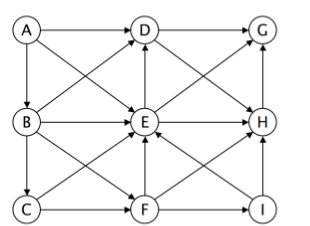
\includegraphics[]{fin-s08-1.png}\\
\begin{enumerate}
\renewcommand{\theenumi}{\Alph{enumi}}
	\item Run \textit{depth-first search}, starting at vertex A. Assume the adjacency lists are in lexicographic order, e.g., when exploring vertex E, consider E-D before E-G or E-H. Complete the list of vertices in \textit{preorder} (the order they are first discovered by DFS).\\

	A B C E D G H F I

	\item Run \textit{breadth-first search}, starting at vertex A. Assume the adjacency lists are in lexicographic order. Complete the list of vertices in the order in which they are enqueued.\\

	A B D E C F G H I

\end{enumerate}


\paragraph{\Large 2. Fall 2008 Final Questions 1a and 1b}\mbox{}\\
Run \textit{depth-first search} on the digraph below, starting at vertex A. As usual, assume the adjacency sets are in lexicographic order, e.g., when exploring vertex F, the algorithm considers the edge $F \rightarrow A$ before $F \rightarrow E$ or $F \rightarrow G$.\\
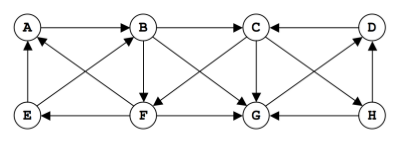
\includegraphics[]{fin-f08-1.png}\\
\begin{enumerate}
\renewcommand{\theenumi}{\Alph{enumi}}
	\item Complete the \textit{preorder} of the vertices (the order in which the vertices are first visited).\\

	A B C F E G D H

	\item Complete the \textit{postorder} of the vertices (the order in which the vertices are last visited).\\

	E G D F H C B A

\end{enumerate}


\paragraph{\Large 3. Fall 2010 Final Question 3a}\mbox{}\\\
Run \textit{depth-first search} on the digraph below, starting at vertex A. Assume the adjacency lists are in sorted order: for example, when exploring vertex F, the algorithm considers the edge $F \rightarrow C$ before $F \rightarrow E$ or $F \rightarrow H$.\\
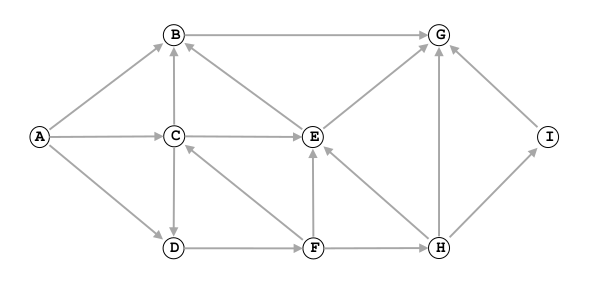
\includegraphics[]{fin-f10-3a.png}\\
List the vertices in preorder and postorder.\\

	preorder: A B G C D F E H I\\
\indent
	postorder: G B E I H F D C A\\

\end{document}